%% BioMed_Central_Tex_Template_v1.06
%%                                      %
%  bmc_article.tex            ver: 1.06 %
%                                       %

%%IMPORTANT: do not delete the first line of this template
%%It must be present to enable the BMC Submission system to
%%recognise this template!!

%%%%%%%%%%%%%%%%%%%%%%%%%%%%%%%%%%%%%%%%%
%%                                     %%
%%  LaTeX template for BioMed Central  %%
%%     journal article submissions     %%
%%                                     %%
%%          <8 June 2012>              %%
%%                                     %%
%%                                     %%
%%%%%%%%%%%%%%%%%%%%%%%%%%%%%%%%%%%%%%%%%


%%%%%%%%%%%%%%%%%%%%%%%%%%%%%%%%%%%%%%%%%%%%%%%%%%%%%%%%%%%%%%%%%%%%%
%%                                                                 %%
%% For instructions on how to fill out this Tex template           %%
%% document please refer to Readme.html and the instructions for   %%
%% authors page on the biomed central website                      %%
%% http://www.biomedcentral.com/info/authors/                      %%
%%                                                                 %%
%% Please do not use \input{...} to include other tex files.       %%
%% Submit your LaTeX manuscript as one .tex document.              %%
%%                                                                 %%
%% All additional figures and files should be attached             %%
%% separately and not embedded in the \TeX\ document itself.       %%
%%                                                                 %%
%% BioMed Central currently use the MikTex distribution of         %%
%% TeX for Windows) of TeX and LaTeX.  This is available from      %%
%% http://www.miktex.org                                           %%
%%                                                                 %%
%%%%%%%%%%%%%%%%%%%%%%%%%%%%%%%%%%%%%%%%%%%%%%%%%%%%%%%%%%%%%%%%%%%%%

%%% additional documentclass options:
%  [doublespacing]
%  [linenumbers]   - put the line numbers on margins

%%% loading packages, author definitions

%\documentclass[twocolumn]{bmcart}
% uncomment this for twocolumn layout and comment line below
\documentclass{bmcart}

%%% Load packages
%\usepackage{amsthm,amsmath}
%\RequirePackage{natbib}
%\RequirePackage{hyperref}
\usepackage[utf8]{inputenc} %unicode support
\usepackage{graphicx}
\usepackage{multirow}
%\usepackage[applemac]{inputenc} %applemac support if unicode package fails
%\usepackage[latin1]{inputenc} %UNIX support if unicode package fails


%%%%%%%%%%%%%%%%%%%%%%%%%%%%%%%%%%%%%%%%%%%%%%%%%
%%                                             %%
%%  If you wish to display your graphics for   %%
%%  your own use using includegraphic or       %%
%%  includegraphics, then comment out the      %%
%%  following two lines of code.               %%
%%  NB: These line *must* be included when     %%
%%  submitting to BMC.                         %%
%%  All figure files must be submitted as      %%
%%  separate graphics through the BMC          %%
%%  submission process, not included in the    %%
%%  submitted article.                         %%
%%                                             %%
%%%%%%%%%%%%%%%%%%%%%%%%%%%%%%%%%%%%%%%%%%%%%%%%%


%\def\includegraphic{}
%\def\includegraphics{}



%%% Put your definitions there:
\startlocaldefs
\endlocaldefs


%%% Begin ...
\begin{document}

%%% Start of article front matter
\begin{frontmatter}

\begin{fmbox}
\dochead{Software}

%%%%%%%%%%%%%%%%%%%%%%%%%%%%%%%%%%%%%%%%%%%%%%
%%                                          %%
%% Enter the title of your article here     %%
%%                                          %%
%%%%%%%%%%%%%%%%%%%%%%%%%%%%%%%%%%%%%%%%%%%%%%

\title{gnparser: a Powerful Scientific Names Parser}

%%%%%%%%%%%%%%%%%%%%%%%%%%%%%%%%%%%%%%%%%%%%%%
%%                                          %%
%% Enter the authors here                   %%
%%                                          %%
%% Specify information, if available,       %%
%% in the form:                             %%
%%   <key>={<id1>,<id2>}                    %%
%%   <key>=                                 %%
%% Comment or delete the keys which are     %%
%% not used. Repeat \author command as much %%
%% as required.                             %%
%%                                          %%
%%%%%%%%%%%%%%%%%%%%%%%%%%%%%%%%%%%%%%%%%%%%%%

\author[
   addressref={aff1},
   corref={aff1},                       % id of corresponding address, if any
   email={dmozzherin@illinois.edu}
]{\inits{DYM}\fnm{Dmitry Y.} \snm{Mozzherin}}
\author[                  % id's of addresses, e.g. {aff1,aff2}
   noteref={n1},% id's of article notes, if any
   email={alexander.myltsev@phystech.edu}   % email address
]{\inits{AAM}\fnm{Alexander A.} \snm{Myltsev}}
\author[
   email={dpatterson.mbl@gmail.com}
]{\inits{DJP}\fnm{David J.} \snm{Patterson}}

%%%%%%%%%%%%%%%%%%%%%%%%%%%%%%%%%%%%%%%%%%%%%%
%%                                          %%
%% Enter the authors' addresses here        %%
%%                                          %%
%% Repeat \address commands as much as      %%
%% required.                                %%
%%                                          %%
%%%%%%%%%%%%%%%%%%%%%%%%%%%%%%%%%%%%%%%%%%%%%%

\address[id=aff1]{%                    % unique id
  \orgname{University of Illinois},    % university, etc
  \street{1816 South Oak St.},         %
  \city{Champaign},                    % city
  \state{IL},
  \postcode{61820},
  \cny{US}                             % country
}

%%%%%%%%%%%%%%%%%%%%%%%%%%%%%%%%%%%%%%%%%%%%%%
%%                                          %%
%% Enter short notes here                   %%
%%                                          %%
%% Short notes will be after addresses      %%
%% on first page.                           %%
%%                                          %%
%%%%%%%%%%%%%%%%%%%%%%%%%%%%%%%%%%%%%%%%%%%%%%

\begin{artnotes}
%\note{Sample of title note}     % note to the article
\note[id=n1]{Equal contributor} % note, connected to author
\end{artnotes}

\end{fmbox}% comment this for two column layout

%%%%%%%%%%%%%%%%%%%%%%%%%%%%%%%%%%%%%%%%%%%%%%
%%                                          %%
%% The Abstract begins here                 %%
%%                                          %%
%% Please refer to the Instructions for     %%
%% authors on http://www.biomedcentral.com  %%
%% and include the section headings         %%
%% accordingly for your article type.       %%
%%                                          %%
%%%%%%%%%%%%%%%%%%%%%%%%%%%%%%%%%%%%%%%%%%%%%%

\begin{abstractbox}

\begin{abstract} % abstract
  \parttitle{Background}
  Modern biology is unthinkable without names based on Linnaean nomenclature.
  Names of organisms are pervasive, they are metadata which allows to
  communicate information in biodiversity, ecology, molecular biology, medicine
  and many other fields. However indexing and organizing such information via
  scientific names is challenging for several reasons. As an example -- names
  exist in a variety of alternative forms like ``\textit{Aedes (Cancraedes)
  thurmanae}'' and ``\textit{Aedes thurmanae} Mattingly, 1958'', therefore a
  simple string comparison often fails to connect information via names due to
  these variations. Parsing would break names into semantic elements, allowing
  to compare them by their \textit{canonical form} (\textit{Aedes thurmanae}
  for both examples).
  \parttitle{Results}
  We introduce Global Names Parser (\textit{gnparser}) -- a tool based on
  Parsing Expression Grammar algorithm. The parser is able to deal with the
  most complex scientific name strings. It finds semantic meaning for all
  words within a scientific name (like ranks, years of publication, names of
  authors etc.). Global Names Parser is written in Scala, a Java Virtual
  Machine language.  Measured throughput was up to 20 million names/hour per
  CPU. Precision was X, Recall X, F-value X. We show that \textit{gnparser} is
  compatible with Scala, Java, R, Jython, and JRuby.
  \parttitle{Conclusions}
  Global Names Parser (\textit{gnparser}) is a long awaited tool for
  biodiversity informatics. It is released under Open Source MIT license. It
  allows to disassemble scientific names of any complexity into their semantic
  elements. It is scalable to deal with billions of name strings an hour, can
  be directly incorporated by many popular languages. The parser can be used as
  a command line application, socket server, or a web server.
\end{abstract}

%%%%%%%%%%%%%%%%%%%%%%%%%%%%%%%%%%%%%%%%%%%%%%
%%                                          %%
%% The keywords begin here                  %%
%%                                          %%
%% Put each keyword in separate \kwd{}.     %%
%%                                          %%
%%%%%%%%%%%%%%%%%%%%%%%%%%%%%%%%%%%%%%%%%%%%%%

\begin{keyword}
\kwd{biodiversity}
\kwd{scientific name}
\kwd{parser}
\end{keyword}

% MSC classifications codes, if any
%\begin{keyword}[class=AMS]
%\kwd[Primary ]{}
%\kwd{}
%\kwd[; secondary ]{}
%\end{keyword}

\end{abstractbox}
%
%\end{fmbox}% uncomment this for twcolumn layout

\end{frontmatter}

%%%%%%%%%%%%%%%%%%%%%%%%%%%%%%%%%%%%%%%%%%%%%%
%%                                          %%
%% The Main Body begins here                %%
%%                                          %%
%% Please refer to the instructions for     %%
%% authors on:                              %%
%% http://www.biomedcentral.com/info/authors%%
%% and include the section headings         %%
%% accordingly for your article type.       %%
%%                                          %%
%% See the Results and Discussion section   %%
%% for details on how to create sub-sections%%
%%                                          %%
%% use \cite{...} to cite references        %%
%%  \cite{koon} and                         %%
%%  \cite{oreg,khar,zvai,xjon,schn,pond}    %%
%%  \nocite{smith,marg,hunn,advi,koha,mouse}%%
%%                                          %%
%%%%%%%%%%%%%%%%%%%%%%%%%%%%%%%%%%%%%%%%%%%%%%

%%%%%%%%%%%%%%%%%%%%%%%%% start of article main body
% <put your article body there>

\section*{Conventions}

Throughout the paper we distinguish between two terms -- ``name'' and
``name-string''. Term ``name'' varies in its meaning for different
nomenclatural codes. According to botanical code of nomenclature \cite{ICN}
\textit{Pinus silvestris} is considered to be a single name. According to
zoological code \cite{ICZN} \textit{Parus major} is considered to be a
combination of two names -- \textit{Parus} and \textit{major}. In the paper we
use term ``name'' in ``botanical'' sense unless stated otherwise.

The ``name-string'' term represents a sequence of characters (letters, numbers,
punctuation, spaces, symbols) used to represent a name. Both \textit{Pinus
silvestris} and \textit{Parus major} correspond to one name-string each.

A name can be expressed by many name-strings, some are well-formed and code
compliant, and others are not (for example see Table~\ref{table:carex}). There
are millions of scientific names and billions of possible legitimate name
strings.

When we talk about ``code-compliancy'' we mean compliance with a corresponding
code of nomenclature (Zoological \cite{ICZN}, Botanical \cite{ICN},
Bacteria \cite{ICNB}, Viruses \cite{ICTV}, Cultivated plants \cite{ICNCP},
Phylocode \cite{ICPN}). Codes of nomenclature determine rules for composing
scientific names from infraspecific to family level. Other levels comply with
community practices.

\section*{Background}

The names of organisms are invaluable in the world of big biodiversity data
because they can be used as near universal metadata to index, organize and
interconnect distributed information \cite{Patterson2010}. Nevertheless, use of
names for informatics purposes presents an array of problems. As we demonstrate
further many of these problems can be solved by parsing, or deducing the
semantic meaning of words occurred in the name-strings.

\begin{table}[!htb]
  \begin{center}
  \caption{Some legitimate versions of the scientific name for the Northern
    Bulrush or Singlespike sedge.  The genus (Carex), species (scirpoidea), and
    subspecies (convoluta) may be annotated (var. subsp., and ssp.) or have the
    name of the original authority for the infraspecies (Kükenthal), the species
    (Michaux), the current infraspecific combination (Dunlop), sometimes
    abbreviated and with or without dates. Image courtesy of \cite{FNA2002}.
  }\label{table:carex}
    \begin{tabular}{| l | c |}
    \hline
    Carex scirpoidea convoluta &
    \multirow{24}{*}{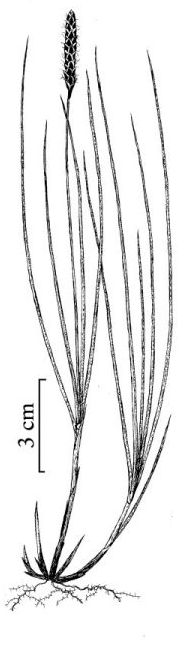
\includegraphics[scale=0.3]{images/carex.png}} \\
    Carex scirpoidea var. convoluta & \\
    Carex scirpoidea subsp. convoluta & \\
    Carex scirpoidea convoluta Kükenth. & \\
    Carex scirpoidea var. convoluta Kuk. & \\
    Carex scirpoidea var. convoluta Kük. & \\
    Carex scirpoidea var. convoluta Kükenth. & \\
    Carex scirpoidea var. convoluta Kükenthal & \\
    Carex scirpoidea Michx. var. convoluta Kük. & \\
    Carex scirpoidea ssp. convoluta (Kük.) Dunlop & \\
    Carex scirpoidea Michx. var. convoluta Kükenth. & \\
    Carex scirpoidea subsp. convoluta (Kük.) Dunlop & \\
    Carex scirpoidea ssp. convoluta (Kukenth.) Dunlop & \\
    Carex scirpoidea Michaux var. convoluta Kükenthal & \\
    Carex scirpoidea subsp. convoluta (Kük.) D.A.Dunlop & \\
    Carex scirpoidea subsp. convoluta (Kük.) D.A. Dunlop & \\
    Carex scirpoidea Michx. ssp. convoluta (Kük.) Dunlop & \\
    Carex scirpoidea subsp. convoluta (Kuk.) D. A. Dunlop & \\
    Carex scirpoidea Michx. subsp. convoluta (Kük.) Dunlop & \\
    Carex scirpoidea Michx. ssp. convoluta (Kükenth.) Dunlop & \\
    Carex scirpoidea subsp. convoluta (Kükenthal) D.A. Dunlop & \\
    Carex scirpoidea Michx. subsp. convoluta (Kük.) D.A.Dunlop & \\
    Carex scirpoidea Michx. subsp. convoluta (Kük.) D.A. Dunlop & \\
    Carex scirpoidea subsp. convoluta (Kükenthal 1909) D.A. Dunlop 1998 & \\
    \hline
    \end{tabular}
  \end{center}
\end{table}

Due to intrinsic diversity of name-strings (Table~\ref{table:carex}) an exact
string matching is not powerful enough to link distributed big data via
scientific names. This problem can be addressed by promoting a rigid standard
restricting each name to a single name-string, or through
\textit{reconciliation}. The former strategy would require a costly
international coordination, would not eliminate future human mistakes, it
cannot be applied to older documents, does not allow for multiple points of
view, nor for changes in taxonomic perspective.

The reconciliation process involves folding of all known name-strings into
lexical groups. This requires that we collate all variant spellings of names.
Parsing in crucial for creating lexical groups of name-strings: it allows to
find the most common denominator of spelling variants -- a canonical form
(\textit{Carex scirpoidea convoluta} in case of Table~\ref{table:carex}) and
extract other important for reconciliation  information (infraspecific ranks,
original and combination authorities etc.). Lexical groups would then require
another level of folding into reconciliation groups where homotypic and
heterotypic synonyms are placed together. This process requires an accurate
database of nomenclatural events (for example Global Names Usage Bank
\cite{Pyle2003}).

Reconciliation uses the most stable component of a name-string -- its canonical
form. Such approach brings us to another problem -- the same canonical form may
be used for more than one taxon or concept in case of homonyms, chresonyms, or
ranks of infraspecies. Analysis of ranks and the authors found by a
parser in name-strings helps to separate homonyms and similar names from each
other.

The next challenge is to replace outdated names with ones that are endorsed by
taxonomic authorities -- this is a process referred to as \textit{resolution}.
Resolution requires an up to date high quality taxonomic and nomenclatural data
to map a reconciled name-string to the currently used name/names. A
reconciliation of name-strings used by a taxonomic authority with name-strings
supplied by user makes parsing a very important step at this stage as well.

A significant number of biodiversity informatics projects (Encyclopedia of Life
\cite{eol}, Global Biodiversity Informatics Facility \cite{gbif}, Catalogue of
Life \cite{col}, World Register of Marine Species \cite{worms}, iDigBio
\cite{idigbio}, VertNet \cite{vertnet} etc.) aggregate information from many
different sources.  Resulting name-strings are inconsistent in their format.
Parsed names can be normalized to the same style. Some name strings are not
properly formed, other contain annotations which are not part of the name.
There are also “surrogate names” -- they depict organisms which were not fully
identified and mapped to a formally described taxon, instead they were
associated with a name string that narrows down identification choices to some
higher clade. Parser helps to recognize such names and mark them as surrogate
name-strings.

After collecting parsed data from a large name-string repository a researcher
can use the data as a basis for statistical analysis, or for practical
purposes. For example parsed data can be used to introduce faceted search by
authors name, year of publication, species epithet etc. If a name-string cannot
be ingested by a high quality parser, the string is almost certainly not a
well-formed scientific name. As a result parser can weed out problematic name
strings from collection.

\subsection*{Prior Art}

Until recently the problem of scientific name parsing had been addressed by
home-grown scripts running regular expressions or by manual splitting of a name
into its canonical form and the authorship part. Both approaches proved to be
limited. Regular expressions are not designed for recursive patterns (and
complex scientific name strings are recursive by nature, as it is most obvious
with hybrid formulae). Manual approach of splitting names into 2 parts is
expensive, slow, inflexible and cannot elegantly deal with name-strings where
authorship is present in the middle of the name.

Names can be quite complex (for example ``\textit{Brassica oleracea} L.
\textit{subsp.  capitata} (L.) DC. \textit{convar. fruticosa} (Metzg.) Alef.
$\times$ \textit{B. oleracea} L.  \textit{subsp. capitata} (L.) \textit{var.
costata} DC.'')  and include authorship for every mentioned taxon, include or
omit infraspecific ranks, original and combination authors etc. Authorship
itself is quite complex and can include original authors who described a name,
authors of a new combination, or authors who made a name, but did not publish
it. We obviously do not want to exclude names from biodiversity informatics
just because they are not simple enough. We need an approach that is able to
deal with names of any complexity.

In 2008 we decided to create a specialized parsing library
``\textit{biodiversity}'' \cite{biodiversity} written in Ruby and based on
Parsing Expression Grammar (PEG) methodology \cite{Ford2004}. We used an
excellent TreeTop Ruby library \cite{treetop} as an underlying PEG
implementation. PEG is well suited for recursive texts with formally defined
grammars. Scientific names follow rules of nomenclatural codes, and therefore
order and capitalization of elements in scientific names are well structured.

We found that PEG approach allows us to solve all these complexity gracefully.
Also PEG gave us enough flexibility to incorporate edge cases and common
mistakes in formation of names. The library \textit{biodiversity} enjoyed
noticeable popularity. At the time of writing it had been downloaded more than
150,000 times \cite{bdiv_downloads}, it is used by many taxon name resolution
projects (for example by Canadian Register of Marine Species (CARMS)
\cite{carms}, the iPlant TNRS \cite{iplant}, World Registry of Marine Species
(WoRMS) \cite{worms}.  According to BioRuby statistics \textit{biodiversity}
parser is the most popular bio-library in Ruby language \cite{biogems}.

We consider \textit{biodiversity} parser library to be a working prototype -- a
playground which allowed us to identify parsing problems and implement
solutions for them. In the process we found that Parsing Expression Grammar is
very well suited for breaking scientific names into semantic elements. In 2015
we decided to use everything we learned and write ``\textit{gnparser}'' a
completely new parser in Scala to achieve significant boost in speed,
scalability and portability of the library. In this manuscript we describe
features, performance and discuss future enhancements of this new parser.

\section*{Implementation}

- written in Scala. What was the reason for the choice

- gnparser consists of three parts. Short description of parts

\subsection*{Parser}

- explanation of functionality: parser engine

- dependency of the rest 2 components on this one

- versions of scala supported

- relation to biodiversity parserj

- relationship to parboiled2, mention Alex' role in paraboiled2

- changes in parboiled2

- optimizations in parser

- input: name string, output: JSON object.

- Figure with output example and short explanation

- Quality output -- short explanation.

- reference to JSON schema (attachment), simple explanation of fields
(attachment)

- short explanations of tests. Connection between tests and schema

- usage with other languages as a library

\subsection*{Runner}

- explanation of functionalilty: command line tool, socket server

- command line tool -- input for one name, output, intput for file, output

- socket server -- very short explanation how it runs. Input, Output

- TODO: should we change input output to be more similar to REST API?
  Make it JSON array of names as input, array of gnparser objects as output

\subsection*{Web}

- explanation of functionality: Web GUI, REST API

- input and output for API use via GET and POST

\subsection*{Installation}

- reference to README. Reference and short explanation of the Docker project
(in attachments)

- MIT license

\subsection*{Testing Material}

- random 100 000 names from 23 million names in GN. Used for performance,
precision tests

- random 1000 names to test Recall

- explanation of quality of the names -- they are from the wild, from sources
of different quality. Good correspondance to what to expect 'in reality'

\section*{Results and Discussion}

To describe parser's use cases, future developments.

\section*{Conclusions}

We introduced \textit{gnparser}, a tool for dissecting scientific name strings
into meaningful parts. Parsing of name strings is necessary component for their
matching, finding them in texts, sharing them in standardised forms,
extracting, comparing and analysing metadata ``hidden'' in the name strings.
The gnparser tool is released under MIT Open Source license, contains command
line executable, socket, web, and REST services, and is optimized for use as a
library in languages like Scala, Java, R, Jyphon, Jruby.

\section*{Availability and Requirements}

Where to find the program etc.

\section*{Abbreviations}

PEG -- Parsing Expression Grammer

\section*{Author's Contributions}

Who did what

\section*{Acknowledgements}

Grant and people to mention

\section*{Leftovers to use in sections above}
Scala is a strongly typed language built from the ground up as a combination of
object oriented and functional programming paradigms. One of the main features
of functional programming is preservation of immutable state, as a result it is
possible to run several parts of program in parallell without danger of
modifying state. Scala creates a rare flexibility of approaches to solve
computational problems. Scala had been written on Java Virtual Machine. It
means that the vast resources developed in Java are easily accessible in Scala.
And vice versa -- the libraries we produce can be used in a plethora of
languages (Java, Jython, Renjin, JRuby etc.). Scala, is a language designed for
scalability. Projects like Akka and Spark create flexibility of approaches in
concurrency and parallelization, allowing to execute code on many CPU and
computers at the same time, dramatically reducing response time for large
computational tasks.

The library parboiled2 had been initiated by one of the authors of this
manuscript, Alexander Myltsev in 2013 while participating in the Google Summer
of Code project initiated by TypeSafe organization. Alexander also had been the
major contributor in gnparser code.

%%%%%%%%%%%%%%%%%%%%%%%%%%%%%%%%%%%%%%%%%%%%%%%%%%%%%%%%%%%%%
%%                  The Bibliography                       %%
%%                                                         %%
%%  Bmc_mathpys.bst  will be used to                       %%
%%  create a .BBL file for submission.                     %%
%%  After submission of the .TEX file,                     %%
%%  you will be prompted to submit your .BBL file.         %%
%%                                                         %%
%%                                                         %%
%%  Note that the displayed Bibliography will not          %%
%%  necessarily be rendered by Latex exactly as specified  %%
%%  in the online Instructions for Authors.                %%
%%                                                         %%
%%%%%%%%%%%%%%%%%%%%%%%%%%%%%%%%%%%%%%%%%%%%%%%%%%%%%%%%%%%%%

% if your bibliography is in bibtex format, use those commands:
\bibliographystyle{bmc-mathphys} % Style BST file
\bibliography{gnparser.bib}      % Bibliography file (usually '*.bib' )

% or include bibliography directly:
% \begin{thebibliography}
% \bibitem{b1}
% \end{thebibliography}

\end{document}
